\chapter{Metody}

V této kapitole popíšeme metody, kterým byl prováděn experiment. Technické detaily,
jako například algoritmus, kterým byl generován šum, nebo hodnoceny lokace, jsou
ale uvedeny až v dokumentaci aplikace, která je druhou přílohou této práce.

\section{Účastníci}

Účastníků bylo celkem deset, pět v každé
skupině. Zrak všech z nich byl normální nebo upravený na normální (např.
brýlemi). Byli vybráni z okolí autora této práce, nejednalo se tedy o náhodný
výběr z populace. Do skupin byli rozřazeni náhodně. Ve skupině se zpětnou
vazbou byl věkový průměr 27 let, dva muži a tři ženy, ve skupině bez zpětné
vazby 26, jeden muž a čtyři ženy. Detailnější statistiky jsou uveden v první
příloze. Za účast na experimentu nebyli účastníci nijak odměněni.

\section{Nástroje a stimuly}
\begin{figure}
\begin{center}
\begin{tabular}{c}
\begin{subfigure}{0.95\textwidth}
\centering
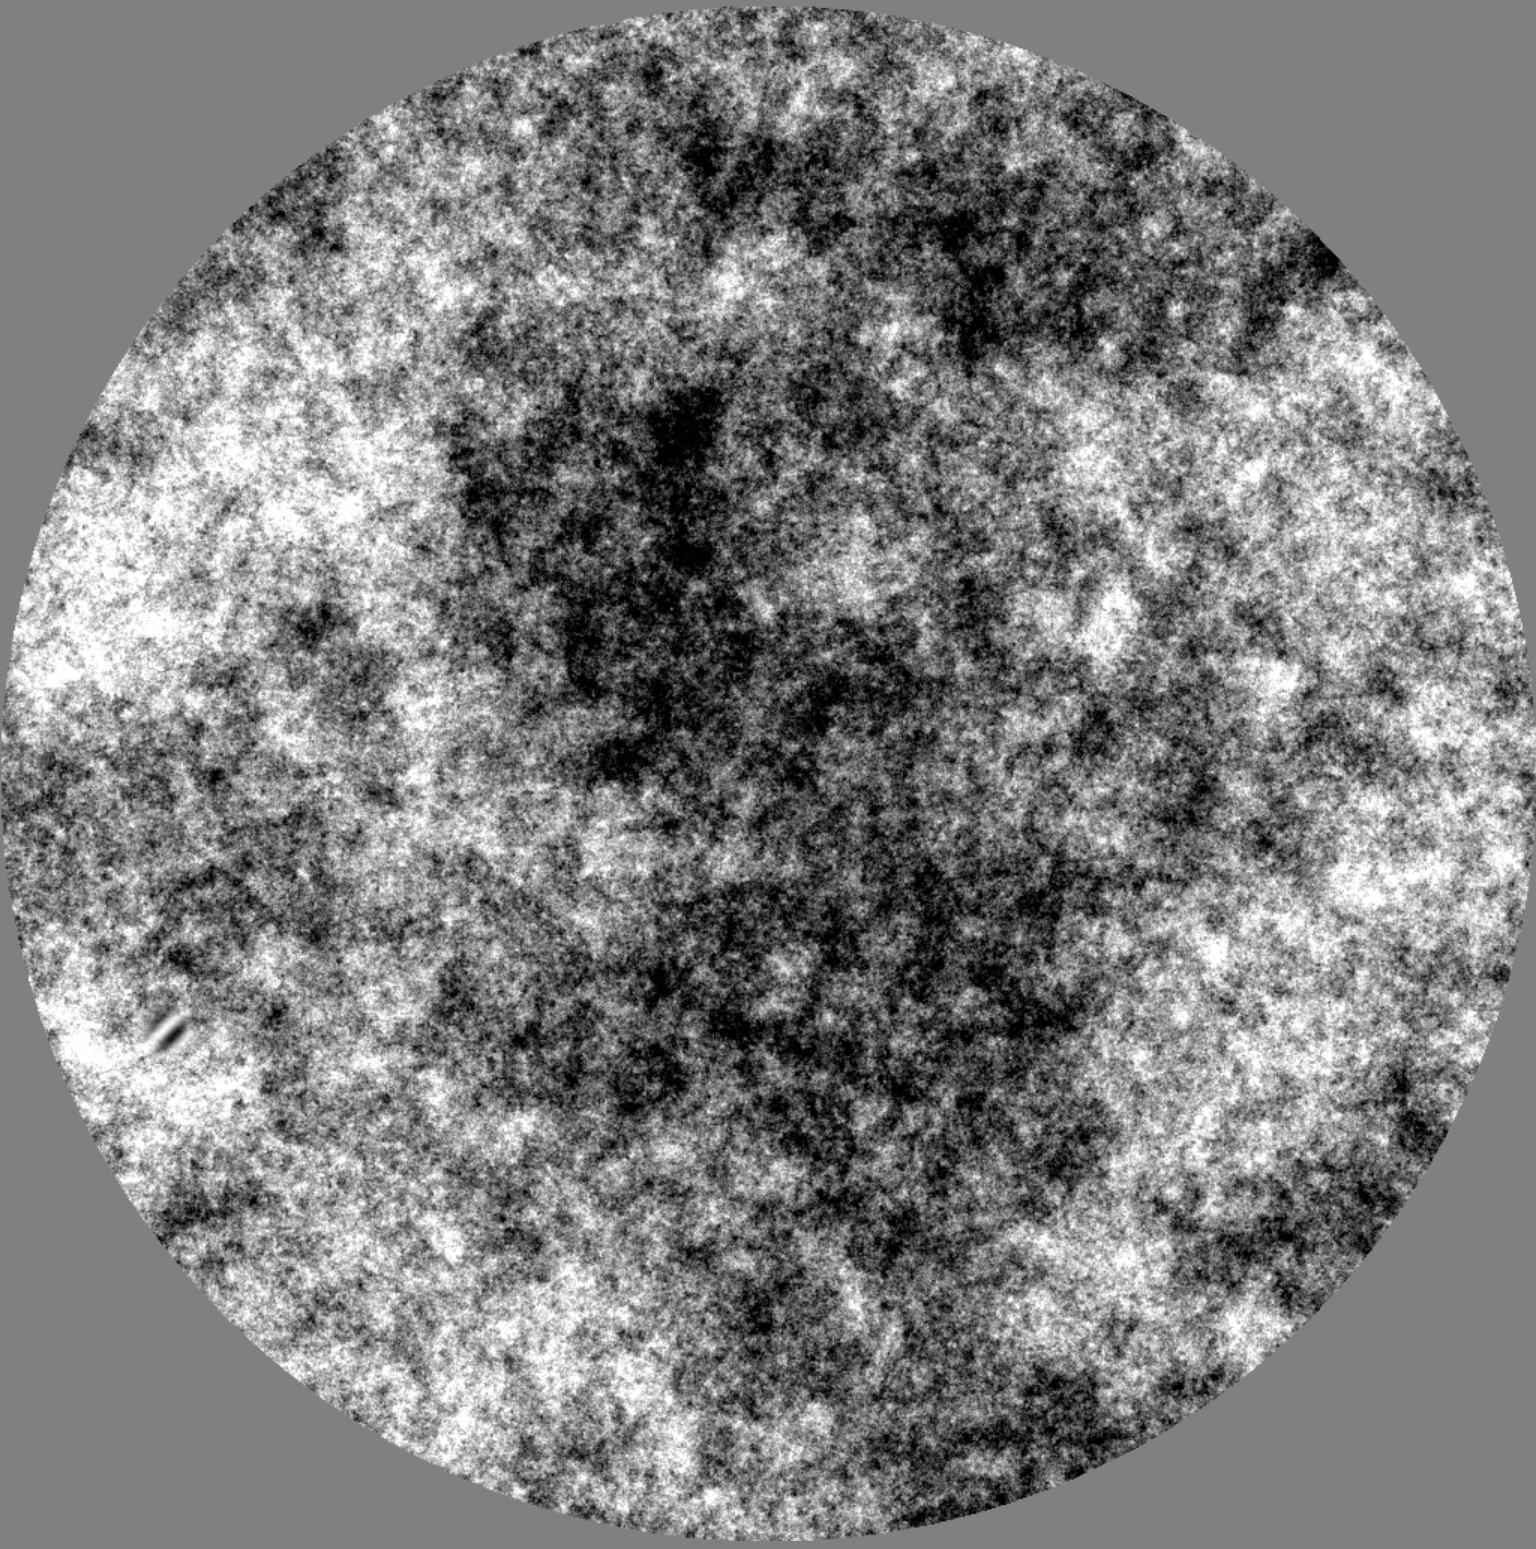
\includegraphics[width = .75\linewidth]{img/noise_visible}
\caption{Šum s dobře viditelným Gabor patchem u levého dolního okraje (kontrast $0.99$).}
\end{subfigure}\\
\noalign{\vskip\bigskipamount}
\\
\begin{subfigure}{0.95\textwidth}
\centering
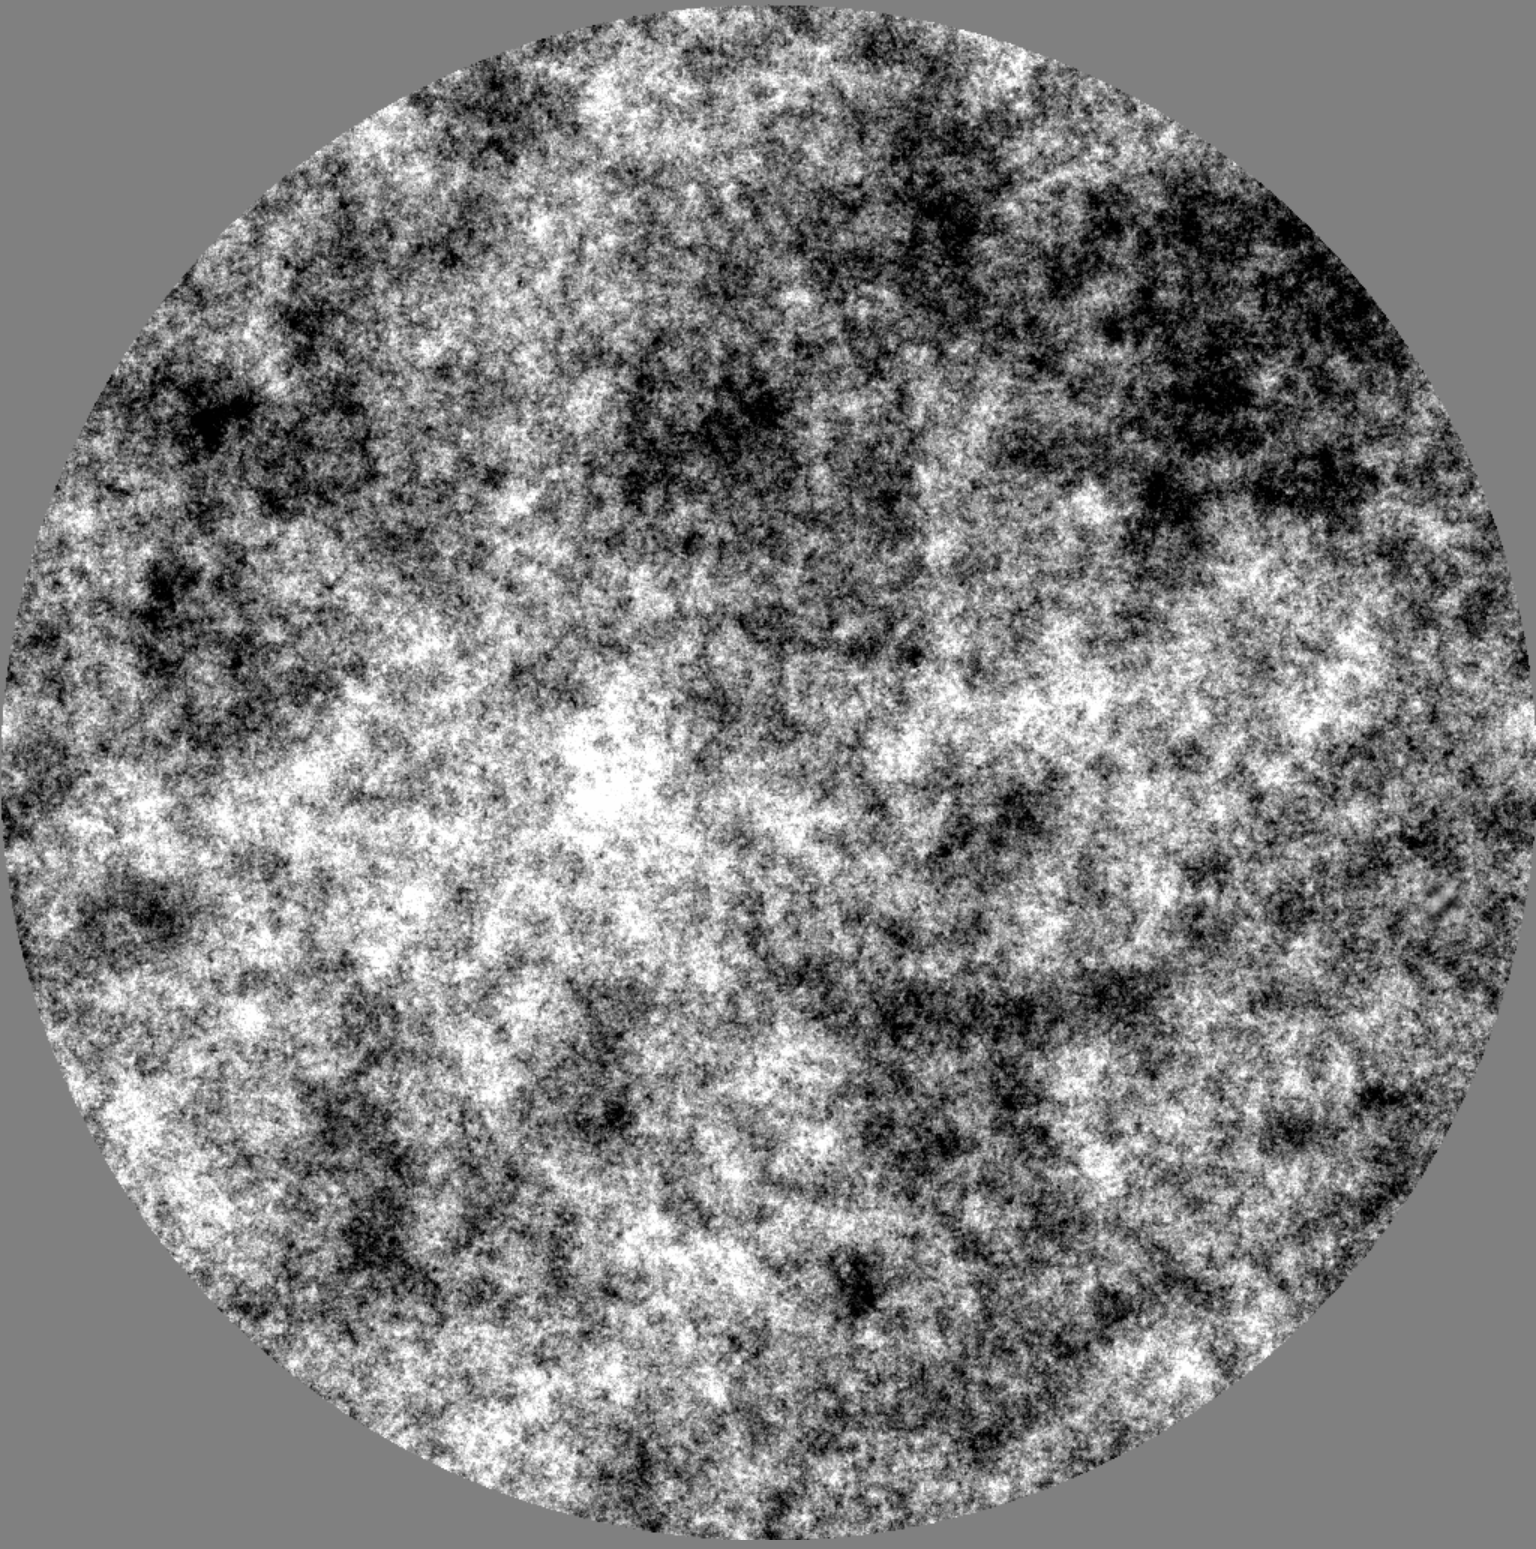
\includegraphics[width = .75\linewidth]{img/noise_invisible}
\caption{Šum se špatně viditelným Gabor patchem u pravého okraje (kontrast $0.61$).}
\end{subfigure}
\end{tabular}
\caption{Příklady šumů s cíli.}
\end{center}
\end{figure}

K experimentu byla použita aplikace, která je součástí této práce. 
Jako zobrazovací zařízení byl použit iPad air s displejem o rozlišení
$2048\times1536$ a o úhlopříčce $9.7$ palců, což odpovídá rozměrům displeje asi
$19.7 \times 14.8$ centimetrů. Hustota pixelů je 264 pixelů na palec. 

V experimentu použitý růžový šum byl kruhový a jeho průměr byl 1024 pixelů.
\footnote{Odsud již všude, kde není zřejmý opak, se pixelem myslí
pixel obrázku, nikoliv pixel displeje.} Tento průměr byl zvolen proto, že je
to nejbližší mocnina dvojky ke kratšímu rozměr displeje iPadu v pixelech.
Mocnina dvojky byla zvolena kvůli použití rychlé Fourierova transformace při
generování růžového šumu. RMS kontast\footnote{{\it RMS kontrast} je pro
černobílý obraz vlastně jiný název pro standarní odchylku jasu pixelu, kdy jas
měříme tak, aby černý pixel dostal hodnotu nula a bílý hodnotu jedna
\citep{RMS}.} šumu byl po vygenerování roven $0.25$, ale při zobrazování byly
hodnoty lišící se od střední hodnoty o více než dvě standardní odchylky
přiblíženy ke střední hodnotě právě na tuto vzdálenost, čímž byl RMS kontrast
mírně snížen. \index{RMS kontrast}

Jako stimulus byl použit Gabor patch. Jedním z problémů aditivního Gabor patche
ale je fakt, že jas pixelu je v praxi omezený. Kdybychom tedy přičítali Gabor
patch k šumu v místě, které má samo o sobě vysoký jas, museli bychom jeho nejvyšší
bod snížit tak, aby součet se šumem nepřesáhl maximální hodnotu jasu pixelu.
Obdobný problém bychom měli s oblastí s nízkým jasem. Tento problém byl vyřešen
tak, že Gabor k šumu nebyl ale přičten k šumu, ale vložen do něj, jako
kdybychom kreslili Gabor patch přes šum a obálka zastupovala alfa kanál. To
znamená, že jas pixelu v bodě $x$ byl spočítán jako $S[x] * (1-o[x]) +
G[x]*o[x]$, kde $S[x]$ je hodnota šumu v bodě $x$, a $G[x]$ a $o[x]$ jsou
hodnoty Gaboru a jeho obálky.  Zvolené parametry Gabor patche byly:

\begin{itemize}
\item Obálka: Raised cosine
\item Průměr: 50 pixelů
\item Frekvence: $1/16$ cyklu na pixel
\item Fázový posun: 0
\item Úhel $\Theta$: $135^\circ$ 
\end{itemize}

\begin{figure}
\centering
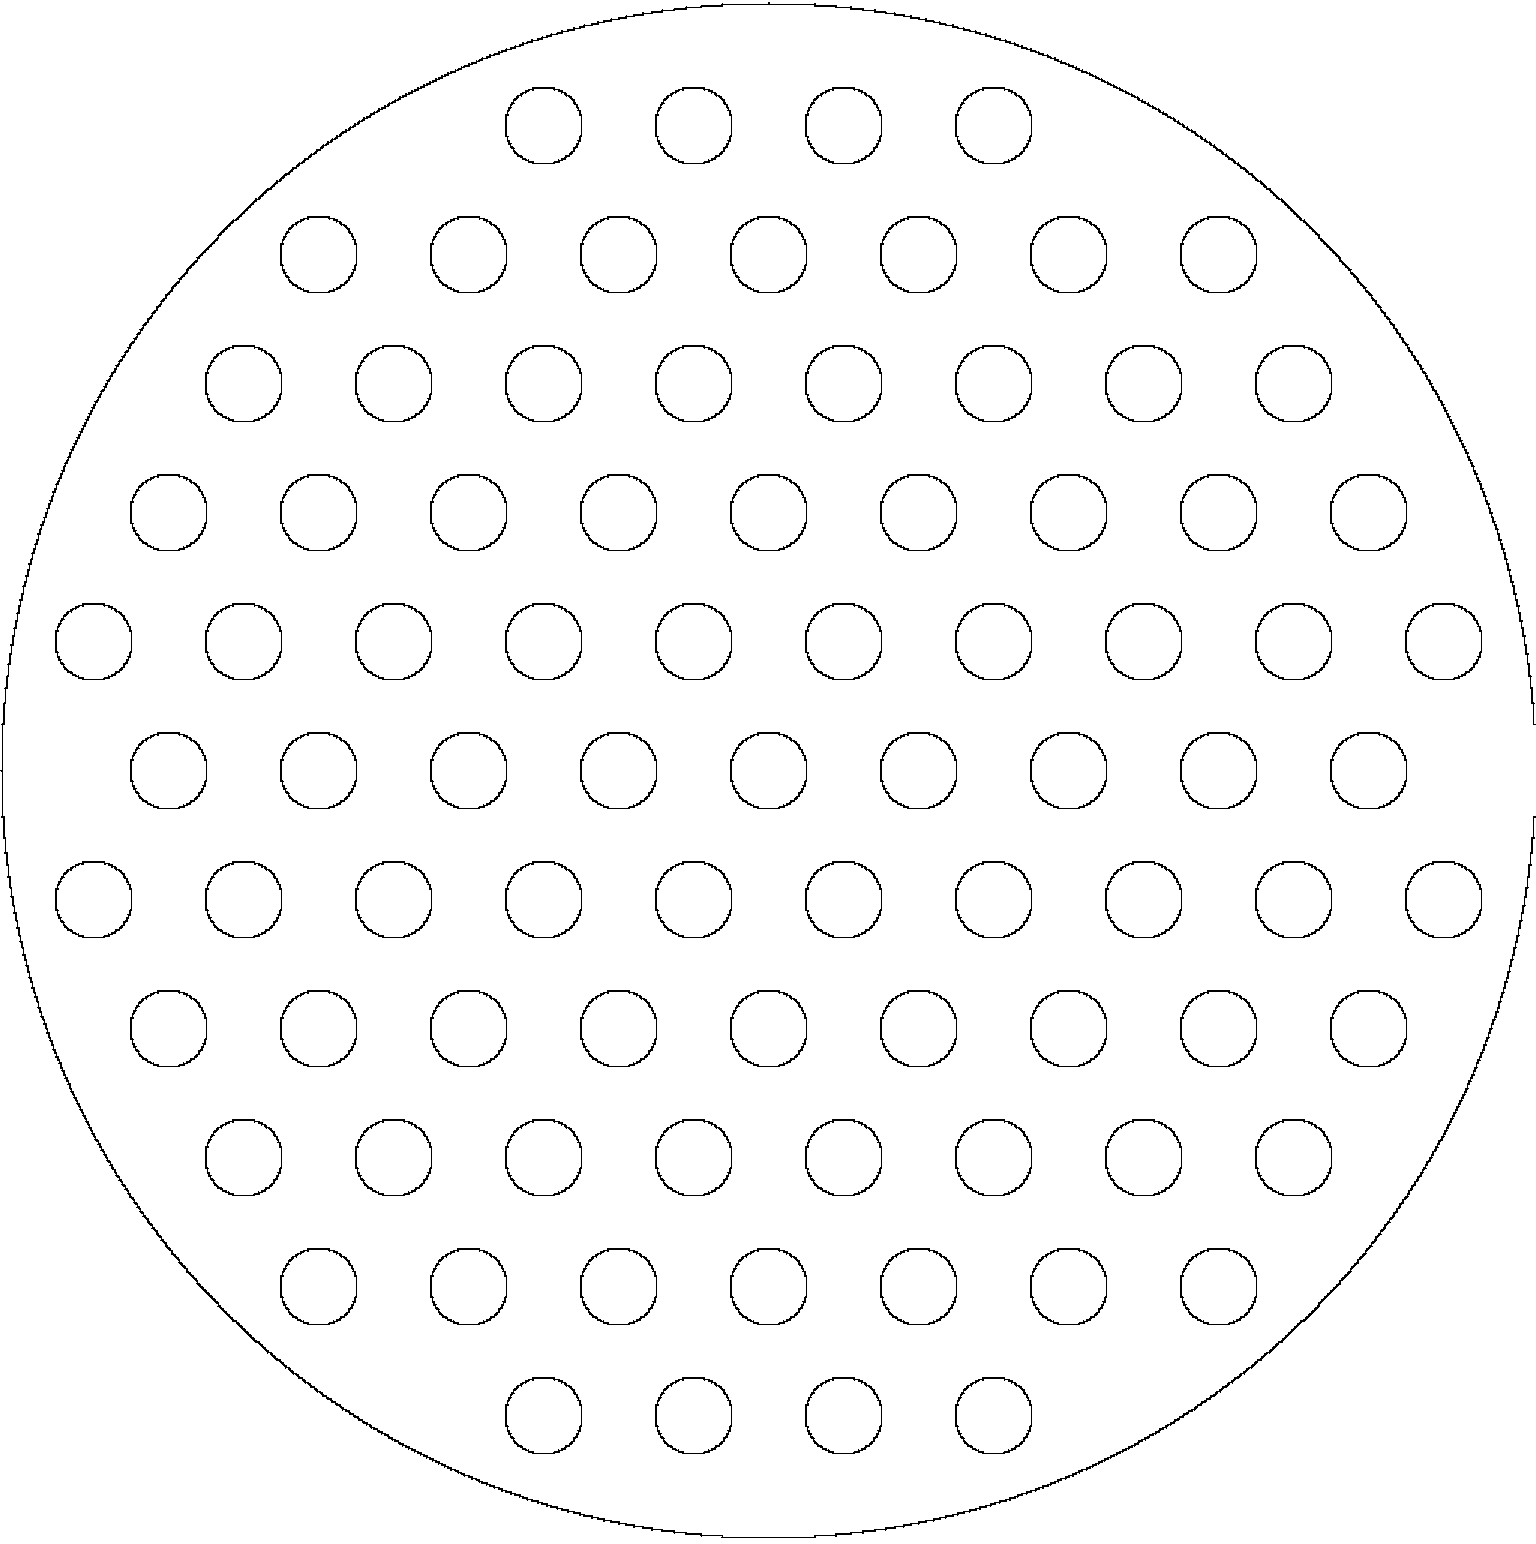
\includegraphics[width=0.48\textwidth]{img/locations_outline.png}
\caption {Možné lokace Gabor patche}.
\end{figure}

Možných lokací Gabor patche bylo celkem 85, a byly rozmístěny po scéně v
trojúhelníkové mřížce tak, aby jedna možná lokace byla ve středu. Vzdálenost
dvou sousedních možných lokací byla 100 pixelů. 

Kontrast cíle byl daný maximem obálky, tedy při snižování kontrastu byl cíl čím dál tím průhlednější. Hodnoty kontrastu se mohly pohybovat mezi nulou a jedničkou.

\section{Procedura}

Každý subjekt prošel sadou 3
testů. V prvním testu mu bylo postupně prezentováno 40 úkolů, kde
v každém z nich měl najít Gabor patch v růžovém šumu.  
V druhém testu bylo prezentováno 120 obdobných úkolů a ve třetím opět 40. Ve druhém testu dostávaly
subjekty, které byly ve skupině se zpětnou vazbou, po každé fixaci zvukovou
odpověď, která značila, kolik informace mohli od této fixace očekávat (tedy
jestli bylo z pohledu ELM moudré udělat právě tuto fixaci). Tato odpověď
byla ve formě tónu, jehož frekvence $f$ byla dána vzorcem
$$f = 440\operatorname{Hz}*2^{2-2*\frac{c - \delta}{\Delta - \delta}},$$ kde $c$ je očekávané snížení entropie při fixaci, kterou si subjekt vybral, $\Delta$ je maximální dosažitelné očekávané
snížení entropie a $\delta$ minimální v případě, že by byla zafixována některá
z možných lokací cíle.\footnote{To znamená, že je potenciálně možné dosáhnout
výsledku lepšího než $\Delta$, resp. horšího, než $\delta$. Rozdíl by však
neměl být důležitý.} 

V každém úkolu byl šum překryt černou barvou. Subjekt se měl vždy dotknout displeje v místě, které se
rozhodl zafixovat. Na tomto místě byl poté šum odkryt na $300
\operatorname{ms}$. Výpočet tvaru a míry odkrytí oblasti bylo provedeno
vynásobením s $d'$ mapou posunutou do bodu fixace, s parametrem $d'_0$
nastaveným na 1 a ostatními parametry naměřenými na pozorovateli FD
($e_R=223$, $e_L=223$, $e_U = 161$, $e_D = 164$, $\beta=2.46$, všechny
veličiny, u nichž má smysl uvádět jednotku, jsou v pixelech).

Ve chvíli, kdy si subjekt myslel, že objevil cíl, zmáčkl tlačítko. Poté mu byl ukázán celý odkrytý šum, ovšem
bez cíle. Potom se měl subjekt dotknout šumu na místě, kde si myslel, že se cíl
nacházel. Cíl byl považován za nalezený, pokud byla vzdálenost vybraného místa
a středu skutečné lokace cíle menší než 60 pixelů displeje. Úkol byl považován za úspěšně splněný, pokud byl cíl nalezen a současně v rámci něj účastník provedl nejvýše šest fixací. 

V každém testu byl počáteční kontrast cíle $0.7$. Pokaždé, když byl subjekt třikrát po sobě úspěšný,
byla zvýšena obtížnost snížením kontrastu cíle o $0.01$, pokud byl
třikrát po sobě neúspěšný, byla obtížnost opět snížena. 

Byl tedy využit obecný postup, kterému se říká Up/Down metoda. Tento postup se používá,
pokud je závislost pravděpodobnosti daného jevu na nějakém parametru rostoucí
(či obecně monotónní) funkce. Spočívá v tom, že se daný parametr snižuje, když
jev nastává, a zvyšuje když nenastává (v obou případech o předem danou
konstantu, která se během experimentu nemění, nemusí však být v obou směrech
stejná). Blíže je popsána v knize Psychophysics: A practical introduction \citep{psychophysics}.
Na rozdíl od implementace této metody, která je popsaná v knize, jsme se
rozhodli za jev považovat tři úspěchy za sebou a za jeho absenci tři neúspěchy,
abychom zmenšili velký rozptyl, který náš jev jinak má.\TODO{Nebo jak tohle okecat?}

Hodnota $0.01$ byla vybrána tak, aby se během 120 úkolů, které jsou v
prostředním testu, účastník mohl teoreticky dostat až na hodnoty kontrastu
kolem $0.3$. S kontrastem menším než přibližně $0.45$ je ale pravděpodobnost
splnění úkolu bez ohledu na strategii podle subjektivního názoru autora práce
velmi nízká. V experimentu se tento dojem potvrdil, nejnižší v experimentu
dosažený kontrast byl $0.51$.



\section{Limitace}

Při návrhu experimentu jsme narazili na několik problémů, které mohou vnést
nepřesnosti do měření, ale jejichž řešení je mimo rozsah této práce. Konkrétně
se jedná o následující obtíže:

\begin{itemize}
\item Vjemy lidského pozorovatele neodpovídají příliš dobře vjemům simulovaného
ideálního pozorovatele. Aby si tyto vjemy odpovídaly, alespoň přibližné, museli
bychom každému pozorovateli změřit jeho vlastní $d'$ mapu. Měření $d'$ mapy ale
i  v té nejminimalističtější variantě, která se používá, trvá nejméně jeden
pracovní den. Druhým důvodem, proč mohou být vjemy rozdílné i v případě, že by
konstanty $d'$ mapy vyšly pozorovateli stejně, jaké byly použity, je, že tato
naměřená $d'$ mapa odpovídá situaci, kdy je scéna se šumem umístěna tak daleko
od pozorovatele, aby ji viděl pod zorným úhlem $15^\circ$. To při velikosti
scény v našem případě odpovídá vzdálenosti pozorovatele a zařízení přibližně
$65 \operatorname{cm}$. V našich experimentech nebyla vzdálenost pozorovatele od
scény hlídána. a určitě byla nižší, než řečených $65 \operatorname{cm}$
(dodržení této vzdálenosti by odpovídalo situaci, kdy by subjekty držely iPad
před sebou zhruba na délku natažené paže). 

\item I pokud odhlédneme od nepřesností zmíněných v předchozím bodě a dovolíme
si na chvíli (evidentně scestný) předpoklad, že subjekty měly vlastní $d'$ mapu
konstantní, narazíme na další problém. Okraj oblasti, která byla odkrývána,
byl ztmavován lineárně se snižující se hodnotou $d'$ v použité $d'$ mapě.
Závislost $d'$ na kontrastu ale téměř jistě
není lineární.

\item S tím souvisí ještě jeden problém: Subjekty samozřejmě nemají svou $d'$
mapu konstantní. Tato mapa se tedy nějak skládá s $d'$ mapou, pomocí které
bylo určeno odhalování šumu. V práci jsme toto skládání ignorovali (tedy
předpokládali jsme, že $d'$ na kontrastu závisí lineárně a $d'$ mapa subjektů
je konstantní.) Nabízela by se otázka, proč tedy bylo zatemňování šumu vůbec
prováděno. To se dělo z několika důvodů:

\begin{itemize}

\item Zatemňování šumu zavádí potřebu klikat na místa, která chce pozorovat v
dalším kroku prozkoumat. Nutí tedy pozorovatele, aby tato rozhodnutí dělal
vědomě a nikoli podvědomě, což byl jeden z efektů, které jsme chtěli zkoumat.

\item Celý proces jedné fixace tímto způsobem také trvá mnohem déle (nižší
jednotky vteřin místo nižších desetin vteřiny) a poskytuje nám tedy mnoho času
na update mapy aposteriorních pravděpodobností a výpočet množství informace,
kterou lze získat následující fixací.

\item Takto navržený experiment též umožňuje zjišťovat, které lokace subjekt
fixuje bez použití eyetrackeru nebo jiných technologií.

\end{itemize}

\item Je možné, že u lidí, kteří nikdy dříve Gabor patch hledat nezkoušeli, se
během testů mění jejich senzitivita na Gabor patch (mění se hodnota $d'(0,0)$).

\item Vzhledem k tomu, že počet reálných pixelů displeje neodpovídal (a ani
nebyl dělitelný) velikostí scény v pixelech, je možné, že byly efekty jako
například antialiasing změněny lokální kontrasty scény.

\item Ve výzkumu v oblasti psychofyziky se většinou
pečlivě kontroluje prostředí (například se zatemňuje místnost, v níž se provádí experiment). To jsme v našem výzkumu nedělali.

\end{itemize}

Tyto nepřesnosti však nepovažujeme za příliš důležité, protože cílem této práce
není přesný experiment, ale pouze proof of concept. Za zásadní chybu naopak
nepovažujeme malý počet účastníků -- kdybychom chtěli na této práci postavit
přesný experiment, nebylo by potřeba zvyšovat počet účastníků, ale pouze počet
měření na jednotlivých účastnících, například tak, že bychom vícekrát opakovali
první a třetí test. Jinak ale není ve výzkumu nutně přínosné velký vzorek,
často je lepší na malém vzorku provést větší počet přesnějších měření
\citep{SmallN}. Kdybychom se však rozhodli raději pro Large-$N$ design, mohli
bychom většinu ostatních parametrů experimentu ponechat, ale bylo by potřeba
přinejmenším o řád více účastníků. 

